% Created by tikzDevice version 0.12.3.1 on 2021-05-09 13:07:40
% !TEX encoding = UTF-8 Unicode
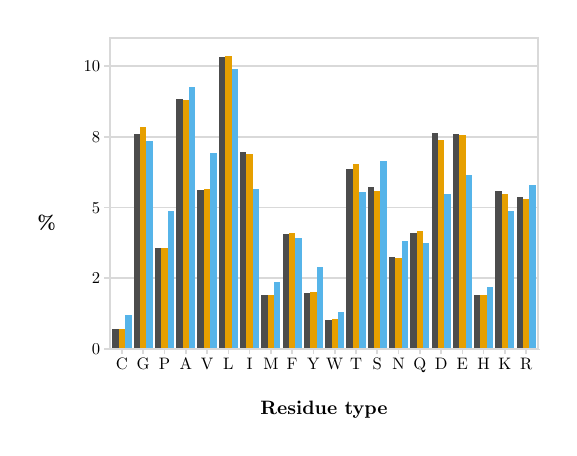
\begin{tikzpicture}[x=1pt,y=1pt]
\definecolor{fillColor}{RGB}{255,255,255}
\path[use as bounding box,fill=fillColor,fill opacity=0.00] (0,0) rectangle (188.25,144.54);
\begin{scope}
\path[clip] ( 29.46, 28.30) rectangle (184.75,141.04);
\definecolor{drawColor}{gray}{0.85}

\path[draw=drawColor,line width= 0.6pt,line join=round] ( 29.46, 28.53) --
	(184.75, 28.53);

\path[draw=drawColor,line width= 0.6pt,line join=round] ( 29.46, 54.05) --
	(184.75, 54.05);

\path[draw=drawColor,line width= 0.6pt,line join=round] ( 29.46, 79.57) --
	(184.75, 79.57);

\path[draw=drawColor,line width= 0.6pt,line join=round] ( 29.46,105.09) --
	(184.75,105.09);

\path[draw=drawColor,line width= 0.6pt,line join=round] ( 29.46,130.61) --
	(184.75,130.61);
\definecolor{fillColor}{RGB}{86,180,233}

\path[fill=fillColor] ( 58.29, 28.53) rectangle ( 60.59,123.05);

\path[fill=fillColor] (181.29, 28.53) rectangle (183.60, 87.73);

\path[fill=fillColor] (135.16, 28.53) rectangle (137.47, 67.32);

\path[fill=fillColor] (150.54, 28.53) rectangle (152.85, 84.57);

\path[fill=fillColor] ( 35.22, 28.53) rectangle ( 37.53, 40.57);

\path[fill=fillColor] (142.85, 28.53) rectangle (145.16, 66.81);

\path[fill=fillColor] (158.23, 28.53) rectangle (160.53, 91.41);

\path[fill=fillColor] ( 42.91, 28.53) rectangle ( 45.22,103.66);

\path[fill=fillColor] (165.92, 28.53) rectangle (168.22, 50.88);

\path[fill=fillColor] ( 81.35, 28.53) rectangle ( 83.66, 86.10);

\path[fill=fillColor] ( 73.66, 28.53) rectangle ( 75.97,129.69);

\path[fill=fillColor] (173.60, 28.53) rectangle (175.91, 78.34);

\path[fill=fillColor] ( 89.04, 28.53) rectangle ( 91.34, 52.62);

\path[fill=fillColor] ( 96.73, 28.53) rectangle ( 99.03, 68.44);

\path[fill=fillColor] ( 50.60, 28.53) rectangle ( 52.91, 78.34);

\path[fill=fillColor] (127.48, 28.53) rectangle (129.78, 96.21);

\path[fill=fillColor] (119.79, 28.53) rectangle (122.10, 85.18);

\path[fill=fillColor] (112.10, 28.53) rectangle (114.41, 41.80);

\path[fill=fillColor] (104.41, 28.53) rectangle (106.72, 58.13);

\path[fill=fillColor] ( 65.98, 28.53) rectangle ( 68.28, 99.27);
\definecolor{fillColor}{RGB}{230,159,0}

\path[fill=fillColor] ( 32.92, 28.53) rectangle ( 35.22, 35.64);

\path[fill=fillColor] ( 40.61, 28.53) rectangle ( 42.91,108.49);

\path[fill=fillColor] ( 48.29, 28.53) rectangle ( 50.60, 64.95);

\path[fill=fillColor] ( 55.98, 28.53) rectangle ( 58.29,118.26);

\path[fill=fillColor] ( 63.67, 28.53) rectangle ( 65.98, 86.28);

\path[fill=fillColor] ( 71.36, 28.53) rectangle ( 73.66,134.25);

\path[fill=fillColor] ( 79.04, 28.53) rectangle ( 81.35, 98.71);

\path[fill=fillColor] ( 86.73, 28.53) rectangle ( 89.04, 48.07);

\path[fill=fillColor] ( 94.42, 28.53) rectangle ( 96.73, 70.28);

\path[fill=fillColor] (102.11, 28.53) rectangle (104.41, 48.96);

\path[fill=fillColor] (109.80, 28.53) rectangle (112.10, 39.19);

\path[fill=fillColor] (117.48, 28.53) rectangle (119.79, 95.16);

\path[fill=fillColor] (125.17, 28.53) rectangle (127.48, 85.39);

\path[fill=fillColor] (132.86, 28.53) rectangle (135.16, 61.40);

\path[fill=fillColor] (140.55, 28.53) rectangle (142.85, 71.17);

\path[fill=fillColor] (148.23, 28.53) rectangle (150.54,104.04);

\path[fill=fillColor] (155.92, 28.53) rectangle (158.23,105.82);

\path[fill=fillColor] (163.61, 28.53) rectangle (165.92, 48.07);

\path[fill=fillColor] (171.30, 28.53) rectangle (173.60, 84.50);

\path[fill=fillColor] (178.99, 28.53) rectangle (181.29, 82.72);
\definecolor{fillColor}{gray}{0.30}

\path[fill=fillColor] ( 30.61, 28.53) rectangle ( 32.92, 35.79);

\path[fill=fillColor] ( 38.30, 28.53) rectangle ( 40.61,106.25);

\path[fill=fillColor] ( 45.99, 28.53) rectangle ( 48.29, 64.92);

\path[fill=fillColor] ( 53.67, 28.53) rectangle ( 55.98,118.59);

\path[fill=fillColor] ( 61.36, 28.53) rectangle ( 63.67, 85.71);

\path[fill=fillColor] ( 69.05, 28.53) rectangle ( 71.36,133.87);

\path[fill=fillColor] ( 76.74, 28.53) rectangle ( 79.04, 99.51);

\path[fill=fillColor] ( 84.43, 28.53) rectangle ( 86.73, 47.79);

\path[fill=fillColor] ( 92.11, 28.53) rectangle ( 94.42, 69.86);

\path[fill=fillColor] ( 99.80, 28.53) rectangle (102.11, 48.79);

\path[fill=fillColor] (107.49, 28.53) rectangle (109.80, 39.01);

\path[fill=fillColor] (115.18, 28.53) rectangle (117.48, 93.35);

\path[fill=fillColor] (122.86, 28.53) rectangle (125.17, 86.89);

\path[fill=fillColor] (130.55, 28.53) rectangle (132.86, 61.55);

\path[fill=fillColor] (138.24, 28.53) rectangle (140.55, 70.19);

\path[fill=fillColor] (145.93, 28.53) rectangle (148.23,106.58);

\path[fill=fillColor] (153.62, 28.53) rectangle (155.92,106.16);

\path[fill=fillColor] (161.30, 28.53) rectangle (163.61, 47.79);

\path[fill=fillColor] (168.99, 28.53) rectangle (171.30, 85.42);

\path[fill=fillColor] (176.68, 28.53) rectangle (178.99, 83.33);

\path[draw=drawColor,line width= 1.1pt,line join=round,line cap=round] ( 29.46, 28.30) rectangle (184.75,141.04);
\end{scope}
\begin{scope}
\path[clip] (  0.00,  0.00) rectangle (188.25,144.54);
\definecolor{drawColor}{RGB}{0,0,0}

\node[text=drawColor,anchor=base east,inner sep=0pt, outer sep=0pt, scale=  0.60] at ( 26.21, 26.46) {0};

\node[text=drawColor,anchor=base east,inner sep=0pt, outer sep=0pt, scale=  0.60] at ( 26.21, 51.98) {2};

\node[text=drawColor,anchor=base east,inner sep=0pt, outer sep=0pt, scale=  0.60] at ( 26.21, 77.50) {5};

\node[text=drawColor,anchor=base east,inner sep=0pt, outer sep=0pt, scale=  0.60] at ( 26.21,103.02) {8};

\node[text=drawColor,anchor=base east,inner sep=0pt, outer sep=0pt, scale=  0.60] at ( 26.21,128.54) {10};
\end{scope}
\begin{scope}
\path[clip] (  0.00,  0.00) rectangle (188.25,144.54);
\definecolor{drawColor}{gray}{0.85}

\path[draw=drawColor,line width= 0.6pt,line join=round] ( 27.71, 28.53) --
	( 29.46, 28.53);

\path[draw=drawColor,line width= 0.6pt,line join=round] ( 27.71, 54.05) --
	( 29.46, 54.05);

\path[draw=drawColor,line width= 0.6pt,line join=round] ( 27.71, 79.57) --
	( 29.46, 79.57);

\path[draw=drawColor,line width= 0.6pt,line join=round] ( 27.71,105.09) --
	( 29.46,105.09);

\path[draw=drawColor,line width= 0.6pt,line join=round] ( 27.71,130.61) --
	( 29.46,130.61);
\end{scope}
\begin{scope}
\path[clip] (  0.00,  0.00) rectangle (188.25,144.54);
\definecolor{drawColor}{gray}{0.85}

\path[draw=drawColor,line width= 0.6pt,line join=round,line cap=rect] ( 29.46, 28.30) --
	(184.75, 28.30);
\end{scope}
\begin{scope}
\path[clip] (  0.00,  0.00) rectangle (188.25,144.54);
\definecolor{drawColor}{gray}{0.85}

\path[draw=drawColor,line width= 0.6pt,line join=round] ( 34.07, 26.55) --
	( 34.07, 28.30);

\path[draw=drawColor,line width= 0.6pt,line join=round] ( 41.76, 26.55) --
	( 41.76, 28.30);

\path[draw=drawColor,line width= 0.6pt,line join=round] ( 49.45, 26.55) --
	( 49.45, 28.30);

\path[draw=drawColor,line width= 0.6pt,line join=round] ( 57.13, 26.55) --
	( 57.13, 28.30);

\path[draw=drawColor,line width= 0.6pt,line join=round] ( 64.82, 26.55) --
	( 64.82, 28.30);

\path[draw=drawColor,line width= 0.6pt,line join=round] ( 72.51, 26.55) --
	( 72.51, 28.30);

\path[draw=drawColor,line width= 0.6pt,line join=round] ( 80.20, 26.55) --
	( 80.20, 28.30);

\path[draw=drawColor,line width= 0.6pt,line join=round] ( 87.89, 26.55) --
	( 87.89, 28.30);

\path[draw=drawColor,line width= 0.6pt,line join=round] ( 95.57, 26.55) --
	( 95.57, 28.30);

\path[draw=drawColor,line width= 0.6pt,line join=round] (103.26, 26.55) --
	(103.26, 28.30);

\path[draw=drawColor,line width= 0.6pt,line join=round] (110.95, 26.55) --
	(110.95, 28.30);

\path[draw=drawColor,line width= 0.6pt,line join=round] (118.64, 26.55) --
	(118.64, 28.30);

\path[draw=drawColor,line width= 0.6pt,line join=round] (126.32, 26.55) --
	(126.32, 28.30);

\path[draw=drawColor,line width= 0.6pt,line join=round] (134.01, 26.55) --
	(134.01, 28.30);

\path[draw=drawColor,line width= 0.6pt,line join=round] (141.70, 26.55) --
	(141.70, 28.30);

\path[draw=drawColor,line width= 0.6pt,line join=round] (149.39, 26.55) --
	(149.39, 28.30);

\path[draw=drawColor,line width= 0.6pt,line join=round] (157.08, 26.55) --
	(157.08, 28.30);

\path[draw=drawColor,line width= 0.6pt,line join=round] (164.76, 26.55) --
	(164.76, 28.30);

\path[draw=drawColor,line width= 0.6pt,line join=round] (172.45, 26.55) --
	(172.45, 28.30);

\path[draw=drawColor,line width= 0.6pt,line join=round] (180.14, 26.55) --
	(180.14, 28.30);
\end{scope}
\begin{scope}
\path[clip] (  0.00,  0.00) rectangle (188.25,144.54);
\definecolor{drawColor}{RGB}{0,0,0}

\node[text=drawColor,anchor=base,inner sep=0pt, outer sep=0pt, scale=  0.60] at ( 34.07, 20.92) {C};

\node[text=drawColor,anchor=base,inner sep=0pt, outer sep=0pt, scale=  0.60] at ( 41.76, 20.92) {G};

\node[text=drawColor,anchor=base,inner sep=0pt, outer sep=0pt, scale=  0.60] at ( 49.45, 20.92) {P};

\node[text=drawColor,anchor=base,inner sep=0pt, outer sep=0pt, scale=  0.60] at ( 57.13, 20.92) {A};

\node[text=drawColor,anchor=base,inner sep=0pt, outer sep=0pt, scale=  0.60] at ( 64.82, 20.92) {V};

\node[text=drawColor,anchor=base,inner sep=0pt, outer sep=0pt, scale=  0.60] at ( 72.51, 20.92) {L};

\node[text=drawColor,anchor=base,inner sep=0pt, outer sep=0pt, scale=  0.60] at ( 80.20, 20.92) {I};

\node[text=drawColor,anchor=base,inner sep=0pt, outer sep=0pt, scale=  0.60] at ( 87.89, 20.92) {M};

\node[text=drawColor,anchor=base,inner sep=0pt, outer sep=0pt, scale=  0.60] at ( 95.57, 20.92) {F};

\node[text=drawColor,anchor=base,inner sep=0pt, outer sep=0pt, scale=  0.60] at (103.26, 20.92) {Y};

\node[text=drawColor,anchor=base,inner sep=0pt, outer sep=0pt, scale=  0.60] at (110.95, 20.92) {W};

\node[text=drawColor,anchor=base,inner sep=0pt, outer sep=0pt, scale=  0.60] at (118.64, 20.92) {T};

\node[text=drawColor,anchor=base,inner sep=0pt, outer sep=0pt, scale=  0.60] at (126.32, 20.92) {S};

\node[text=drawColor,anchor=base,inner sep=0pt, outer sep=0pt, scale=  0.60] at (134.01, 20.92) {N};

\node[text=drawColor,anchor=base,inner sep=0pt, outer sep=0pt, scale=  0.60] at (141.70, 20.92) {Q};

\node[text=drawColor,anchor=base,inner sep=0pt, outer sep=0pt, scale=  0.60] at (149.39, 20.92) {D};

\node[text=drawColor,anchor=base,inner sep=0pt, outer sep=0pt, scale=  0.60] at (157.08, 20.92) {E};

\node[text=drawColor,anchor=base,inner sep=0pt, outer sep=0pt, scale=  0.60] at (164.76, 20.92) {H};

\node[text=drawColor,anchor=base,inner sep=0pt, outer sep=0pt, scale=  0.60] at (172.45, 20.92) {K};

\node[text=drawColor,anchor=base,inner sep=0pt, outer sep=0pt, scale=  0.60] at (180.14, 20.92) {R};
\end{scope}
\begin{scope}
\path[clip] (  0.00,  0.00) rectangle (188.25,144.54);
\definecolor{drawColor}{RGB}{0,0,0}

\node[text=drawColor,anchor=base,inner sep=0pt, outer sep=0pt, scale=  0.70] at (107.10,  4.86) {\bfseries Residue type};
\end{scope}
\begin{scope}
\path[clip] (  0.00,  0.00) rectangle (188.25,144.54);
\definecolor{drawColor}{RGB}{0,0,0}

\node[text=drawColor,anchor=base,inner sep=0pt, outer sep=0pt, scale=  0.70] at (  6.85, 71.44) {\bfseries \%};
\end{scope}
\end{tikzpicture}%
